\documentclass[11pt]{article}
\usepackage[hmargin=1in,vmargin=1in]{geometry}
\usepackage{xcolor}
\usepackage{amsmath}
\usepackage{graphicx} % Required for inserting images
\usepackage{amsmath,amssymb,amsfonts,url,sectsty,framed,tcolorbox,framed}
\usepackage{nicematrix}
\usepackage{amssymb}
\usepackage{algorithm2e}
\setcounter{MaxMatrixCols}{16}
\usepackage{tikz}
\usepackage{hyperref}
\usetikzlibrary{decorations.pathreplacing}
\newcommand{\pf}{{\bf Proof: }}
\newtheorem{theorem}{Theorem}
\newtheorem{lemma}{Lemma}
\newtheorem{proposition}{Proposition}
\newtheorem{definition}{Definition}
\newtheorem{remark}{Remark}
\newcommand{\zbar}{\raisebox{0.2ex}{--}\kern-0.6em Z}
\newcommand{\qed}{\hfill \rule{2mm}{2mm}}
\usepackage{titlesec}

\setcounter{secnumdepth}{4}
\titleclass{\subsubsubsection}{straight}[\subsection]
\newcounter{subsubsubsection}[subsubsection]
\renewcommand{\thesubsubsubsection}{\thesubsubsection.\arabic{subsubsubsection}}
\titleformat{\subsubsubsection}{\normalfont\normalsize\bfseries}{\thesubsubsubsection}{1em}{}
\titlespacing*{\subsubsubsection}{0pt}{3.25ex plus 1ex minus .2ex}{1.5ex plus .2ex}



\begin{document}
%%%%%%%%%%%%%%%%%%%%%%%%%%%%%%%%%%%%%%%%%%%%%%%%%%%%%%%%%%%%%%%%%%%%%
\noindent
\rule{\textwidth}{1pt}
\begin{center}
{\bf [CS304] Introduction to Cryptography and Network Security}
\end{center}
Course Instructor: Dr. Dibyendu Roy \hfill Winter 2023-2024\\
Scribed by: Manas Jitendrakumar Ingle (202151086) \hfill [Week 10]
\\
\rule{\textwidth}{1pt}
%%%%%%%%%%%%%%%%%%%%%%%%%%%%%%%%%%%%%%%%%%%%%%%%%%%%%%%%%%%
%write here

\section{System of Modular Equations}
We will be solving a system of linear equations of the kind, where we have to find x, such that,
\begin{center}
    $a \cdot x \equiv b \ mod \ m$    (Eq.1)
\end{center}
Let us first look at the solution of the above equation. The above equation can be written as,
\begin{center}
    $a \cdot x - m \cdot y = b$     (Eq.2)
\end{center}
where y is an integer. From Bezout's Identiy we know that, 
\begin{center}
    $a \cdot x_0 + m \cdot y_0 = gcd(a, m)$    (Eq.3)
\end{center}
where $x_0$ and $y_0$ can be found using Extended Euclidean Algorithm.

The equation 2 is solvable iff gcd(a, m) divides b, otherwise it will not have a solution. Since, gcd(a, m) divides b, we can say,
\begin{center}
    $t \cdot gcd(a, m) = b$
\end{center}
Multiplying Eq.3 by t, we get, 
\begin{center}
    $a \cdot (t \cdot x_0) + m \cdot (t\cdot y_0) = t \cdot gcd(a, m) \implies a \cdot  X_0 + m \cdot Y_0 = b$
\end{center}

Therefore, given a equation to solve, first we will check if gcd(a, m) divides b or not. If it is dividing then only a solution exists. Then, we will find $x_0$ and $y_0$ using Extended Euclidean Algorithm, and multiply them by $t = \frac{b}{gcd(a, m)}$, to get $X_0$ and $Y_0$.\\
\newline
If we know that $X_0$ and $Y_0$ are a solution of the Eq.2, then we can substitute x and y as, 
\begin{center}
    $x = X_0 + \frac{m}{gcd(a, m)} \cdot n$\\
    \vspace{1mm}
    $y = Y_0 + \frac{a}{gcd(a, m} \cdot n$
\end{center}
where n is an integer. For any value of n, the above x and y will satisfy the Eq.2. Hence, x and y are general solution for the Eq.2.\\
\newline
Now, let us consider a system of two modular equations,
\begin{center}
    $x \equiv a_1 \ mod \ m_1$   (Eq.1)\\
    $x \equiv a_2 \ mod \ m_2$   (Eq.2)  
\end{center}
where $m_1$ and $m_2$ are co-prime. We need to find $x$ that satisfies both the equations. If $x$ is a solution of Eq.1, then.
\begin{center}
    $x = a_1 + m_1 \cdot y$  (Eq.3)
\end{center}
If $x$ is also a solution to Eq.2, then,
\begin{center}
    $x \equiv a_2 \ mod \ m_2$
\end{center}
Let us substitute the value of $x$ from Eq.3,
\begin{center}
    $a_1 + m_1 \cdot y \equiv a_2 \ mod \ m_2 \implies m_1 \cdot y \equiv (a_2 - a_1) \ mod \ m_2$   (Eq.4)
\end{center}
Since, gcd(m1, m2) = 1, therefore, from the general solution for only one equation above, we can say Eq.4 has the solution,
\begin{center}
    $y = y_0 + \frac{m_2}{gcd(m_1, m_2)} \cdot n \implies y = y_0 + m_2 \cdot n$
\end{center}
From Eq.3 we have, 
\begin{center}
    $x = a_1 + m_1 \cdot y \implies x = a_1 + m_1 \cdot (y_0 + m_2 \cdot n)$\\
    \vspace{1mm}
    $\implies x = (a_1 + m_1 \cdot y_0) + n \cdot m_1 \cdot m_2$
\end{center}
If we have $y_0$, let's say $x_0 = a_1 + m_1 \cdot y_0$, then,
\begin{center}
    $x = x_0 + m_1 \cdot m_2 \cdot n$\\
    \vspace{1mm}
    $x \equiv x_0 \ mod \ m_1 \cdot m_2$
\end{center}
$x_0$ is congruent modulo to any $x$ under modulo $m_1 \cdot m_2$. Since, $x$ is the general solution of the two equations, that means, every solution of the given system of equations, will always be congruent to $x_0$ under modulo $m_1 \cdot m_2$.

\subsection{Chinese Remainder Theorem}
Consider the system of equations, 
\begin{center}
    $x \equiv a_1 \ mod \ m_1$\\
    $x \equiv a_2 \ mod \ m_2$\\
    .\\
    .\\
    $x \equiv a_r \ mod \ m_r$\\
\end{center}
where $m_1, m_2, \hdots, m_r$ are pairwise co-prime, then the above system has a unique solution modulo $(m_1 \cdot m_2 \hdots m_r)$. The proof for the above result is given below. For each $1 \leq j \leq r$, define $\delta_j$ as,
\begin{center}
    $\delta_j =$ 
     \begin{cases}
       \text{1,} &\quad\text{$mod \ m_j$}\\
       \text{0,} &\quad\text{$mod \ m_i, \ if\ i \neq j$}\\
     \end{cases}
\end{center}
Now, we can say that $x = \sum_{j=1}^r a_j \cdot \delta_j$ will satisfy the given system of equations. We are claiming that $x$ will satisfy all the equations. Let us expand $x$,
\begin{center}
    $x = \delta_1 \cdot a_1 + \delta_2 \cdot a_2 + \hdots + \delta_r \cdot a_r$ (Eq. 1)
\end{center}
Now, consider the $j^{th}$ equation in the given system of equations,
\begin{center}
    $x \equiv a_j \ mod \ m_j$
\end{center}
If we take modulus of $x$ under $m_j$, we will get,
\begin{center}
    $x \equiv (\delta_1 \cdot a_1 + \delta_2 \cdot a_2 + \hdots + \delta_r \cdot a_r) \ mod \ m_j$
\end{center}
All the $\delta_i, \ for \ i \neq j$ will be 0, and also, $\delta_j = 1$, from the definition of $\delta$. Therefore, 
\begin{center}
    $x \equiv a_j \ mod \ m_j$
\end{center}
Hence, we can conclude that $x$ is a solution of the system of equations, given that we know $\delta_j$. Now, let us find $\delta_j \ for \ 1 \leq j \leq r$. Let us say the integer M is equal to:
\begin{center}
    $M = m_1 \cdot m_2 \hdots m_r$
\end{center}
We want to compute the $gcd(\frac{M}{m_j}, m_j)$. Clearly, it will be equal to 1 because $m_i$ are pairwise co-prime. $M$ is product of all $m_i$, therefore, $\frac{M}{m_j}$ does not contain $m_j$. Hence,
\begin{center}
    $gcd(\frac{M}{m_j}, m_j) = 1$
\end{center}
This means that we can find the inverse of $\frac{M}{m_j}$ under modulo $m_j$. Let $b_j$ be the multiplicative inverse of $\frac{M}{m_j}$ under modulo $m_j$. Then, 
\begin{center}
    $\frac{M}{m_j} \cdot b_j \equiv 1 \ mod \ m_j$
\end{center}
We can use the Extended Euclidean Algorithm to find $b_j$. Now, $delta_j$ is defined as:
\begin{center}
    $\delta_j = \frac{M}{m_j} \cdot b_j$
\end{center}
Clearly, if we divide $\delta_j$ by $m_j$, we will get 1 as remainder. Also, if we take $\delta_j$ and divide it by any $m_i, i \neq j$, then remainder will be 0. We can check it as follows.
\begin{center}
    $\delta_j \ mod \ m_i = \frac{M}{m_j} \cdot b_j \ (mod \ m_i)$\\
    \vspace{1mm}
    $\delta_j \ mod \ m_i = \{\frac{m_1 \cdot m_2 \hdots m_{j-1} \cdot m_{j+1} \hdots m_i \cdot m_{i+1} \hdots m_r}{m_j} \cdot b_j\} \ mod \ m_i$\\
    \vspace{1mm}
    $\delta_j \ mod \ m_i = t \cdot m_i \ (mod \ m_i) = 0$
\end{center}
Therefor, the solution is $x = \sum_{j=1}^r a_j \cdot \delta_j$, where $\delta_j$ is,
\begin{center}
    $\delta_j =$ 
     \begin{cases}
       \text{1,} &\quad\text{$mod \ m_j$}\\
       \text{0,} &\quad\text{$mod \ m_i, \ if\ i \neq j$}\\
     \end{cases}
\end{center}

To solve a given system of equations, follow the steps:
\begin{enumerate}
    \item Check if $m_i$ are pairwise co-prime. If yes, continue to next step.
    \item Calculate $M = m_1 \cdot m_2 \hdots m_r$
    \item Calculate $b_j$ for each $\frac{M}{m_j}$ under modulo $m_j$.
    \item Calculate $\delta_j = \frac{M}{m_j} \cdot b_j$
    \item Calculate $x = \sum_{j=1}^r a_j \cdot \delta_j$
    \item Optionally, you can verify your solution by putting the value of $x$ in each equation.
\end{enumerate}
Now, we will prove the uniqueness of the solution. Assume $x'$ is another solution of the given system of equations, then we can say from our conclusion on a system of two equations that, if we have a solution $x_0$, then every solution will be congruent to $x_0$. Therefore, 
\begin{center}
    $x' \equiv x \ mod \ (m_1 \cdot m_2 \hdots m_r)$
\end{center}
Since, $x \ and \ x'$ are solutions of the system of equations then for any equation we can say,
\begin{center}
    $x \equiv a_i \ mod \ m_i$\\
    $x' \equiv a_i \ mod \ m_i$
\end{center}
If we subtract the above two equations, we will get,
\begin{center}
    $x' - x \equiv 0 \ mod \ m_i \implies x' \equiv x \ mod \ m_i, 1 \leq i \leq r$
\end{center}
Since, $(x' - x)$ is divisible by each $m_i$ and $m_i$ are pairwise co-prime, we can conclude that,
\begin{center}
    $x' \equiv x \ mod \ (m_1 \cdot m_2 \hdots m_r)$
\end{center}
Hence, the solution is unique under modulo $(m_1 \cdot m_2 \hdots m_r)$.

\section{Elliptic Curve Cryptography}
RSA was extremely elementary, we just have to use Square and Multiply Algorithm. Using the Square and Multiply Algorithm, the computations are extremely easy and the methodical things providing security and correctness are also elementary.\\
\newline
Now, we are going to define cryptography known as Elliptic Curve Cryptography. In this, we are going to do the computations on a curve instead of integers. From there, we will be able to see that we can develop Diffie-Hellman Key Exchange Algorithm and Signature Algorithm which are used presently. The key exchange is done using Elliptic Curve Diffie-Hellman (ECDH) and the signatures are done using Elliptic Curve Digital Signature Algorithm (ECDSA). Instead of RSA, we use Elliptic Curve methods because they provide better security using a relatively smaller prime number than RSA.\\
\newline
Let us understand how things work in Elliptic Curve Cryptography. We will begin with real numbers, from which we will develop a discrete structure because cryptography is always based on discrete systems.\\
\newline
Let us define two numbers a and b such that,
\begin{center}
    $a, b \in \mathbb{R} \ and \ 4a^3 + 27b^2 \neq 0$
\end{center}
Let us define a curve,
\begin{center}
    $y^2 = x^3 + ax + b$
\end{center}
where $(x,y) \in \mathbb{R}_2$. This curve is called as the Elliptic Curve. If we draw the curve, there will be two structures, one is shown below, and the other will be discussed later.
\begin{center}
    \tikzset{every picture/.style={line width=0.75pt}}
    \begin{tikzpicture}[x=0.75pt,y=0.75pt,yscale=-1,xscale=1]
        \draw    (105,213) -- (498,213) ;
        \draw [shift={(500,213)}, rotate = 180] [color={rgb, 255:red, 0; green, 0; blue, 0 }  ][line width=0.75]    (10.93,-3.29) .. controls (6.95,-1.4) and (3.31,-0.3) .. (0,0) .. controls (3.31,0.3) and (6.95,1.4) .. (10.93,3.29)   ;
        \draw [shift={(103,213)}, rotate = 0] [color={rgb, 255:red, 0; green, 0; blue, 0 }  ][line width=0.75]    (10.93,-3.29) .. controls (6.95,-1.4) and (3.31,-0.3) .. (0,0) .. controls (3.31,0.3) and (6.95,1.4) .. (10.93,3.29)   ;
 
        \draw    (292.01,49) -- (292.99,373) ;
        \draw [shift={(293,375)}, rotate = 269.83] [color={rgb, 255:red, 0; green, 0; blue, 0 }  ][line width=0.75]    (10.93,-3.29) .. controls (6.95,-1.4) and (3.31,-0.3) .. (0,0) .. controls (3.31,0.3) and (6.95,1.4) .. (10.93,3.29)   ;
        \draw [shift={(292,47)}, rotate = 89.83] [color={rgb, 255:red, 0; green, 0; blue, 0 }  ][line width=0.75]    (10.93,-3.29) .. controls (6.95,-1.4) and (3.31,-0.3) .. (0,0) .. controls (3.31,0.3) and (6.95,1.4) .. (10.93,3.29)   ;
 
        \draw    (373,320) .. controls (375.42,318.19) and (373,309) .. (371.45,307.24) .. controls (369.91,305.47) and (182,291) .. (182,213) .. controls (182,135) and (364,117) .. (364.24,103.33) .. controls (364.49,89.66) and (360.53,97.04) .. (365,96) ;

        \draw (506,201) node [anchor=north west][inner sep=0.75pt]   [align=left] {x};
        \draw (295,31) node [anchor=north west][inner sep=0.75pt]   [align=left] {y};
        \draw (163,189) node [anchor=north west][inner sep=0.75pt]   [align=left] {A};
    \end{tikzpicture}
\end{center}
At point A, $y = 0 \implies x^3 + ax + b = 0$ (Eq.1). This equation will have three roots and the roots will be either:
\begin{itemize}
    \item three real roots
    \item one real root, two complex roots
\end{itemize}
Eq.1 will have three distinct root iff $4a^3 + 27b^2 \neq 0$ (can be real or complex). If we consider the above curve and put y = 0, we can see that it will have only one real root and two complex roots.\\
\newline
If we consider three real roots of Eq.1, then the curve will look as shown below.
\begin{center}
    \tikzset{every picture/.style={line width=0.75pt}} 
    \begin{tikzpicture}[x=0.75pt,y=0.75pt,yscale=-1,xscale=1]

        \draw    (127,184) -- (520,184) ;
        \draw [shift={(522,184)}, rotate = 180] [color={rgb, 255:red, 0; green, 0; blue, 0 }  ][line width=0.75]    (10.93,-3.29) .. controls (6.95,-1.4) and (3.31,-0.3) .. (0,0) .. controls (3.31,0.3) and (6.95,1.4) .. (10.93,3.29)   ;
        \draw [shift={(125,184)}, rotate = 0] [color={rgb, 255:red, 0; green, 0; blue, 0 }  ][line width=0.75]    (10.93,-3.29) .. controls (6.95,-1.4) and (3.31,-0.3) .. (0,0) .. controls (3.31,0.3) and (6.95,1.4) .. (10.93,3.29)   ;
        \draw    (314.01,20) -- (314.99,344) ;
        \draw [shift={(315,346)}, rotate = 269.83] [color={rgb, 255:red, 0; green, 0; blue, 0 }  ][line width=0.75]    (10.93,-3.29) .. controls (6.95,-1.4) and (3.31,-0.3) .. (0,0) .. controls (3.31,0.3) and (6.95,1.4) .. (10.93,3.29)   ;
        \draw [shift={(314,18)}, rotate = 89.83] [color={rgb, 255:red, 0; green, 0; blue, 0 }  ][line width=0.75]    (10.93,-3.29) .. controls (6.95,-1.4) and (3.31,-0.3) .. (0,0) .. controls (3.31,0.3) and (6.95,1.4) .. (10.93,3.29)   ;
        \draw    (454,285.6) .. controls (454,281.6) and (451,281.6) .. (450,269.6) .. controls (449,257.6) and (347,262) .. (347,184) .. controls (347,106) and (435.76,98.27) .. (436,84.6) .. controls (436.24,70.93) and (433.53,76.64) .. (438,75.6) ; 
        \draw    (157,184) .. controls (197,154) and (210,164.6) .. (257,184) ;
        \draw    (157,184) .. controls (193,212.6) and (209,208.6) .. (257,184) ;

        \draw (528,172) node [anchor=north west][inner sep=0.75pt]   [align=left] {x};
        \draw (323,5) node [anchor=north west][inner sep=0.75pt]   [align=left] {y};
    \end{tikzpicture}
\end{center}
Let us define some properties on the curve we defined before.
\begin{center}
    \tikzset{every picture/.style={line width=0.75pt}} 
    \begin{tikzpicture}[x=0.75pt,y=0.75pt,yscale=-1,xscale=1]
        \draw    (105,213) -- (498,213) ;
        \draw [shift={(500,213)}, rotate = 180] [color={rgb, 255:red, 0; green, 0; blue, 0 }  ][line width=0.75]    (10.93,-3.29) .. controls (6.95,-1.4) and (3.31,-0.3) .. (0,0) .. controls (3.31,0.3) and (6.95,1.4) .. (10.93,3.29)   ;
        \draw [shift={(103,213)}, rotate = 0] [color={rgb, 255:red, 0; green, 0; blue, 0 }  ][line width=0.75]    (10.93,-3.29) .. controls (6.95,-1.4) and (3.31,-0.3) .. (0,0) .. controls (3.31,0.3) and (6.95,1.4) .. (10.93,3.29)   ; 
        \draw    (292.01,49) -- (292.99,373) ;
        \draw [shift={(293,375)}, rotate = 269.83] [color={rgb, 255:red, 0; green, 0; blue, 0 }  ][line width=0.75]    (10.93,-3.29) .. controls (6.95,-1.4) and (3.31,-0.3) .. (0,0) .. controls (3.31,0.3) and (6.95,1.4) .. (10.93,3.29)   ;
        \draw [shift={(292,47)}, rotate = 89.83] [color={rgb, 255:red, 0; green, 0; blue, 0 }  ][line width=0.75]    (10.93,-3.29) .. controls (6.95,-1.4) and (3.31,-0.3) .. (0,0) .. controls (3.31,0.3) and (6.95,1.4) .. (10.93,3.29)   ; 
        \draw    (362,317.4) .. controls (355,310.4) and (360,309.4) .. (347,304.4) .. controls (334,299.4) and (182,291) .. (182,213) .. controls (182,135) and (359.76,119.07) .. (360,105.4) .. controls (360.24,91.73) and (368,91.4) .. (362,94.4) ; 
        \draw [color={rgb, 255:red, 245; green, 166; blue, 35 }  ,draw opacity=1 ]   (217,160) -- (218,267.4) ; 
        \draw [color={rgb, 255:red, 208; green, 2; blue, 27 }  ,draw opacity=1 ]   (362,94.4) -- (217,160) ; 
        \draw [color={rgb, 255:red, 65; green, 117; blue, 5 }  ,draw opacity=1 ]   (275,132.4) -- (275,289.4) ;
        \draw [color={rgb, 255:red, 189; green, 16; blue, 224 }  ,draw opacity=1 ]   (362,94.4) -- (362,317.4) ;
        
        \draw (506,201) node [anchor=north west][inner sep=0.75pt]   [align=left] {x};
        \draw (295,31) node [anchor=north west][inner sep=0.75pt]   [align=left] {y};
        \draw (160,132) node [anchor=north west][inner sep=0.75pt]   [align=left] {$P (x_1, y_1)$};
        \draw (226,103) node [anchor=north west][inner sep=0.75pt]   [align=left] {$Q (x_2, y_2)$};
        \draw (142,269) node [anchor=north west][inner sep=0.75pt]   [align=left] {$-P (x_1, -y_1)$};
        \draw (214,298) node [anchor=north west][inner sep=0.75pt]   [align=left] {$-Q (x_2, -y_2)$};
        \draw (368,79) node [anchor=north west][inner sep=0.75pt]   [align=left] {-R};
        \draw (377,317) node [anchor=north west][inner sep=0.75pt]   [align=left] {R};
    \end{tikzpicture}
\end{center}
If we take two points P and Q on the curve and join them using a straight line, it will cut the curve again at a point, say -R. The point -X is mirror image of X with x-axis as mirror. Alternatively, we can say, the perpendicular from point X on the x-axis will cut the curve again at point -X.
\begin{enumerate}
    \item $P \  \boxed{+}  \ Q = R$. The $\boxed{+}$ operation is a binary operator that is defined as: take the two points, join them using a straight line. The line will cut the curve again at some point. The image of this point on the x-axis is the output point.
    \item $\Theta$ is known as the point of infinity. If we join P and -P, the straight line will be parallel to y-axis. The elliptic curve is infinite curve and we are assuming that the straight line is going to cut the curve at one point which will be the point of infinity.
    \item $P \ \boxed{+} -P = \Theta$
    \item ${P \ \boxed{+} \ \Theta = P}$
    \item $(P \ \boxed{+} \ Q) \ \boxed{+} \ R = P \ \boxed{+} \ (Q \ \boxed{+} \ R)$
    \item $P \ \boxed{+} \ Q = Q \ \boxed{+} \ P$
    
\end{enumerate}
The associativity and commutativity of the $\boxed{+}$ operator can be proved using a graphical tool. We can think of $\Theta$ as an identity element and $-P$ as the inverse of $P$. Hence, the curve with the $\boxed{+}$ operator is forming a commutative group.\\

Suppose, we have to find $P \ \boxed{+} P$, then what we do is that we draw the tangent to the curve at P, and wherever the tangent cuts the curve again, its image is the result, it my result. $P \ \boxed{+} P = R \implies 2P = R$. Let us see in the graph:
\begin{center}
    

\tikzset{every picture/.style={line width=0.75pt}} %set default line width to 0.75pt        

\begin{tikzpicture}[x=0.75pt,y=0.75pt,yscale=-1,xscale=1]
%uncomment if require: \path (0,483); %set diagram left start at 0, and has height of 483

%Straight Lines [id:da532177365763133] 
\draw    (105,268.22) -- (498,268.29) ;
\draw [shift={(500,268.29)}, rotate = 180.01] [color={rgb, 255:red, 0; green, 0; blue, 0 }  ][line width=0.75]    (10.93,-3.29) .. controls (6.95,-1.4) and (3.31,-0.3) .. (0,0) .. controls (3.31,0.3) and (6.95,1.4) .. (10.93,3.29)   ;
\draw [shift={(103,268.22)}, rotate = 0.01] [color={rgb, 255:red, 0; green, 0; blue, 0 }  ][line width=0.75]    (10.93,-3.29) .. controls (6.95,-1.4) and (3.31,-0.3) .. (0,0) .. controls (3.31,0.3) and (6.95,1.4) .. (10.93,3.29)   ;
%Straight Lines [id:da20953626690843463] 
\draw    (292.03,89.34) -- (292.96,442.8) ;
\draw [shift={(292.97,444.8)}, rotate = 269.85] [color={rgb, 255:red, 0; green, 0; blue, 0 }  ][line width=0.75]    (10.93,-3.29) .. controls (6.95,-1.4) and (3.31,-0.3) .. (0,0) .. controls (3.31,0.3) and (6.95,1.4) .. (10.93,3.29)   ;
\draw [shift={(292.02,87.34)}, rotate = 89.85] [color={rgb, 255:red, 0; green, 0; blue, 0 }  ][line width=0.75]    (10.93,-3.29) .. controls (6.95,-1.4) and (3.31,-0.3) .. (0,0) .. controls (3.31,0.3) and (6.95,1.4) .. (10.93,3.29)   ;
%Curve Lines [id:da5778038832019325] 
\draw    (513.17,451.17) .. controls (506.17,443.54) and (466.18,371.6) .. (398.18,358.51) .. controls (330.18,345.42) and (177.98,351.06) .. (178,266.05) .. controls (178.01,181.04) and (321.21,195.02) .. (386.22,140.54) .. controls (451.22,86.06) and (448.22,90.42) .. (501.23,29.4) ;
%Straight Lines [id:da5088539639588137] 
\draw [color={rgb, 255:red, 126; green, 211; blue, 33 }  ,draw opacity=1 ]   (165.2,229.87) -- (422.22,110.03) ;
%Straight Lines [id:da3019672495535983] 
\draw [color={rgb, 255:red, 126; green, 211; blue, 33 }  ,draw opacity=1 ]   (422.22,110.03) -- (421.18,367.23) ;
%Shape: Free Drawing [id:dp6112864843116634] 
\draw  [line width=3] [line join = round][line cap = round] (184.19,290.9) .. controls (184.19,290.9) and (184.19,290.9) .. (184.19,290.9) ;
%Straight Lines [id:da5056241281051979] 
\draw [color={rgb, 255:red, 126; green, 211; blue, 33 }  ,draw opacity=1 ]   (222.21,202.63) -- (512.17,440.27) ;
%Straight Lines [id:da9233543125523616] 
\draw [color={rgb, 255:red, 126; green, 211; blue, 33 }  ,draw opacity=1 ]   (490.23,41.39) -- (494.17,426.1) ;

% Text Node
\draw (508,259.25) node [anchor=north west][inner sep=0.75pt]  [rotate=-0.01] [align=left] {x};
% Text Node
\draw (297.03,73.94) node [anchor=north west][inner sep=0.75pt]  [rotate=-0.01] [align=left] {y};
% Text Node
\draw (202.01,154.57) node [anchor=north west][inner sep=0.75pt]  [rotate=-0.01] [align=left] {P (x1, y1)};
% Text Node
\draw (361.03,81.58) node [anchor=north west][inner sep=0.75pt]  [rotate=-0.01] [align=left] {\mbox{-}R = -2P};
% Text Node
\draw (374.98,385.64) node [anchor=north west][inner sep=0.75pt]  [rotate=-0.01] [align=left] {R = 2P};
% Text Node
\draw (469.97,431.43) node [anchor=north west][inner sep=0.75pt]  [rotate=-0.01] [align=left] {\mbox{-}3P};
% Text Node
\draw (441.03,42.36) node [anchor=north west][inner sep=0.75pt]  [rotate=-0.01] [align=left] {3P};


\end{tikzpicture}
\end{center}

In the above figure, P and P co-incide and we draw the tangent and then find its image. If we have to find 3P, then 3P = $2P \ \boxed{+} P$ as shown in figure. So, for NP, NP = $(N-1)P \ \boxed{+} P$. \\
\subsubsection{Mathematical Aspects}
\underline{Elliptic Curve:}\\
\begin{center}
    $y^2\ =\ x^3+ax+b$\\
    $4a^3+27b^2\ \neq 0$
\end{center}
Let us consider two points P($x_1, y_1$) and Q($x_2, y_2$). We have three cases,
\begin{enumerate}
    \item $x_1\neq x_2$, $y_1\neq y_2$
    \item $x_1= x_2$, $y_1=\  -y_2$
    \item $x_1= x_2$, $y_1= y_2$
    
\end{enumerate}
\begin{center}
    

\tikzset{every picture/.style={line width=0.75pt}} %set default line width to 0.75pt        

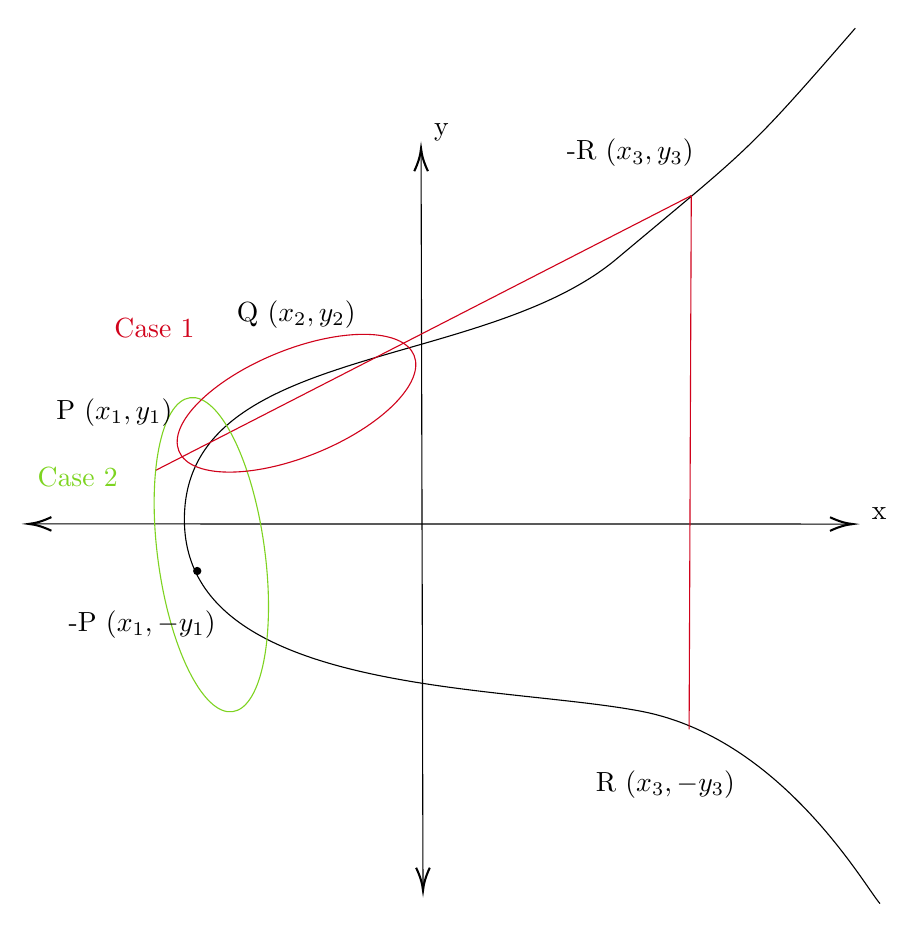
\begin{tikzpicture}[x=0.75pt,y=0.75pt,yscale=-1,xscale=1]
%uncomment if require: \path (0,483); %set diagram left start at 0, and has height of 483

%Straight Lines [id:da532177365763133] 
\draw    (105,268.22) -- (498,268.29) ;
\draw [shift={(500,268.29)}, rotate = 180.01] [color={rgb, 255:red, 0; green, 0; blue, 0 }  ][line width=0.75]    (10.93,-3.29) .. controls (6.95,-1.4) and (3.31,-0.3) .. (0,0) .. controls (3.31,0.3) and (6.95,1.4) .. (10.93,3.29)   ;
\draw [shift={(103,268.22)}, rotate = 0.01] [color={rgb, 255:red, 0; green, 0; blue, 0 }  ][line width=0.75]    (10.93,-3.29) .. controls (6.95,-1.4) and (3.31,-0.3) .. (0,0) .. controls (3.31,0.3) and (6.95,1.4) .. (10.93,3.29)   ;
%Straight Lines [id:da20953626690843463] 
\draw    (292.03,89.34) -- (292.96,442.8) ;
\draw [shift={(292.97,444.8)}, rotate = 269.85] [color={rgb, 255:red, 0; green, 0; blue, 0 }  ][line width=0.75]    (10.93,-3.29) .. controls (6.95,-1.4) and (3.31,-0.3) .. (0,0) .. controls (3.31,0.3) and (6.95,1.4) .. (10.93,3.29)   ;
\draw [shift={(292.02,87.34)}, rotate = 89.85] [color={rgb, 255:red, 0; green, 0; blue, 0 }  ][line width=0.75]    (10.93,-3.29) .. controls (6.95,-1.4) and (3.31,-0.3) .. (0,0) .. controls (3.31,0.3) and (6.95,1.4) .. (10.93,3.29)   ;
%Curve Lines [id:da5778038832019325] 
\draw    (513.17,451.17) .. controls (506.17,443.54) and (466.18,371.6) .. (398.18,358.51) .. controls (330.18,345.42) and (177.98,351.06) .. (178,266.05) .. controls (178.01,181.04) and (321.21,195.02) .. (386.22,140.54) .. controls (451.22,86.06) and (448.22,90.42) .. (501.23,29.4) ;
%Straight Lines [id:da5088539639588137] 
\draw [color={rgb, 255:red, 208; green, 2; blue, 27 }  ,draw opacity=1 ]   (164.2,242.4) -- (422.22,110.03) ;
%Straight Lines [id:da3019672495535983] 
\draw [color={rgb, 255:red, 208; green, 2; blue, 27 }  ,draw opacity=1 ]   (422.22,110.03) -- (421.18,367.23) ;
%Shape: Free Drawing [id:dp6112864843116634] 
\draw  [line width=3] [line join = round][line cap = round] (184.19,290.9) .. controls (184.19,290.9) and (184.19,290.9) .. (184.19,290.9) ;
%Shape: Ellipse [id:dp9247315052804184] 
\draw  [color={rgb, 255:red, 126; green, 211; blue, 33 }  ,draw opacity=1 ] (201.23,358.68) .. controls (187.11,360.59) and (171.08,328.28) .. (165.42,286.51) .. controls (159.75,244.74) and (166.61,209.33) .. (180.73,207.41) .. controls (194.84,205.5) and (210.88,237.81) .. (216.54,279.58) .. controls (222.2,321.35) and (215.35,356.77) .. (201.23,358.68) -- cycle ;
%Shape: Ellipse [id:dp6062445859961849] 
\draw  [color={rgb, 255:red, 208; green, 2; blue, 27 }  ,draw opacity=1 ] (175.36,233.11) .. controls (169.99,219.91) and (191.01,198.9) .. (222.3,186.17) .. controls (253.59,173.45) and (283.31,173.83) .. (288.67,187.03) .. controls (294.04,200.22) and (273.02,221.24) .. (241.73,233.96) .. controls (210.44,246.69) and (180.72,246.31) .. (175.36,233.11) -- cycle ;

% Text Node
\draw (508,259.25) node [anchor=north west][inner sep=0.75pt]  [rotate=-0.01] [align=left] {x};
% Text Node
\draw (297.03,73.94) node [anchor=north west][inner sep=0.75pt]  [rotate=-0.01] [align=left] {y};
% Text Node
\draw (115.01,206.57) node [anchor=north west][inner sep=0.75pt]  [rotate=-0.01] [align=left] {P ($x_1, y_1$)};
% Text Node
\draw (361.03,81.58) node [anchor=north west][inner sep=0.75pt]  [rotate=-0.01] [align=left] {\mbox{-}R ($x_3, y_3$)};
% Text Node
\draw (374.98,385.64) node [anchor=north west][inner sep=0.75pt]  [rotate=-0.01] [align=left] {R ($x_3, -y_3$)};
% Text Node
\draw (202.01,159.57) node [anchor=north west][inner sep=0.75pt]  [rotate=-0.01] [align=left] {Q ($x_2, y_2$)};
% Text Node
\draw (121.01,308.57) node [anchor=north west][inner sep=0.75pt]  [rotate=-0.01] [align=left] {\mbox{-}P ($x_1, -y_1$)};
% Text Node
\draw (143,168) node [anchor=north west][inner sep=0.75pt]   [align=left] {\textcolor[rgb]{0.82,0.01,0.11}{Case 1}};
% Text Node
\draw (106,240) node [anchor=north west][inner sep=0.75pt]   [align=left] {\textcolor[rgb]{0.49,0.83,0.13}{Case 2}};


\end{tikzpicture}
\end{center}
\textbf{\underline{Case-1:}}\\
\begin{center}
    y = mx + c              ...Eqn(a)\\
    m = $\frac{y_2-y_1}{x_2-x_1}$\\
    $y_1$ = $mx_1$ + c\\
    $\implies$ $c = y_1-mx_1$, $c = y_2-mx_2$\\
\end{center}
All the points on this line will satisfy this equation of straight line.\\
Equation of straight line(Eqn(a)) will cut the curve at a point, so we substitute value of y in the curve equation.
\begin{center}
    $y_2=x_3+ax+b$\\
    ${(mx+c)}^2 = x_3+ax+b$\\
    $m^2x^2+2mxc+c^2 = x_3+ax+b$\\
    $x^3-m^2x^2+(a-2mc)x+(b-c^2)=0$\\
\end{center}
We already know that $(x_1,y_1),(x_2,y_2)$ will satisfy this equation.\\
If $x_3$ is another solution of the above system, then\\
\begin{center}
    $x_1+x_2+x_3=m^2$\\
    $\implies$ $x_3=m^2-x_1-x_2$\\
    \vspace{3mm}
    We already know that m = $\frac{y_2-y_1}{x_2-x_1}$ = $\frac{y_3-y_1}{x_3-x_1}$\\
    \vspace{3mm}
    $\implies$ $y_3=y_1+m(x_3-x_1)$\\
\end{center}
So, we see that we obtained co-ordinate of R($x_3,y_3)$
\begin{center}
    $P \ \boxed{+} Q\ =\ R$
\end{center}
\textbf{\underline{Case-2:}}\\
P = $(x_1,y_1)$\\
Q = $(x_2,y_2)$\\
where $x_1=x_2, y_1=-y_2$\\
In this case\\
\begin{center}
    $P \ \boxed{+} Q\ =\ \theta$
\end{center}
\textbf{\underline{Case-3:}}\\
P = $(x_1,y_1)$\\
Q = $(x_2,y_2)$\\
where $x_1=x_2, y_1=y_2$\\
\begin{center}
    $y = mx+c$\\
    $y_2=x_3+ax+b$\\
    $\implies$ $2y\frac{dy}{dx}\ =\ 3x^2+a$\\
    $\implies$ $\frac{dy}{dx}\ =\ \frac{3x^2+a}{2y}$\\
    ${(\frac{dy}{dx})}_{(x_1,y_1)}$ = $\frac{3{x_1}^2+a}{2y_1}$ = m\\
    \vspace{3mm}
    c = $y_1-mx_1$\\
\end{center}
Let us substitute in curve
\begin{center}
    $y_2=x_3+ax+b$\\
    $\implies$${(mx+c)}^2 = x_3+ax+b$\\
    $x_1+x_2+x_3=m^2$\\
    $\implies$$x_3=m^2-x_1-x_2$\\
    $m = \frac{y_3-y_1}{x_3-x_1}$\\
    $\implies$ $y_3 = y_1+m(x_3-x_1)$\\
    R$\rightarrow(x_3,-y_3)$\\
\end{center}
Now, we will be considering the same curve in $\mathbb{Z_P}\ \times\ \mathbb{Z_P}$, where P is a prime number.
\begin{center}
    $y^2=x^3+ax+b$, where (x,y)$\in$ $\mathbb{Z_P}\ \times\ \mathbb{Z_P}$ and a, b $\in\ \mathbb{Z_P}$\\
    $4a^3+27b^2\ \neq\ 0\ mod\ P$\\
\end{center}
Since, we are now working on discrete values, we will not obtain this curve. We will obtain points.\\
\textbf{\underline{Case-1:}}\\
\begin{center}
    $x^3=m^2-x_1-x_2$\\
    $m = \frac{y_2-y_1}{x_2-x_1}$\\
    Now, here we don't divide, we take inverse under mod P\\
    Since $x_2, x_1$ are different values, $x_2-x_1$ will be non-zero and we will be able to find its inverse under mod P since P is prime, so its gcd with ($x_2-x_1)$ will be 1.
    $m = (y_2-y_1)\times{(x_2-x_1)}^{-1}\ mod P$\\
    $\implies$ $y_3=y_1+m(x_3-x_1)\ \in\ \mathbb{Z_P}$\\
\end{center}
\subsubsection{Elliptic Curve Diffie-Hellman(ECDH)}
Let us consider a scenario, where Alice and Bob want to exchange the messages. They have a curve E and a point P and (E, P) is public.
\begin{center}
    


\tikzset{every picture/.style={line width=0.75pt}} %set default line width to 0.75pt        

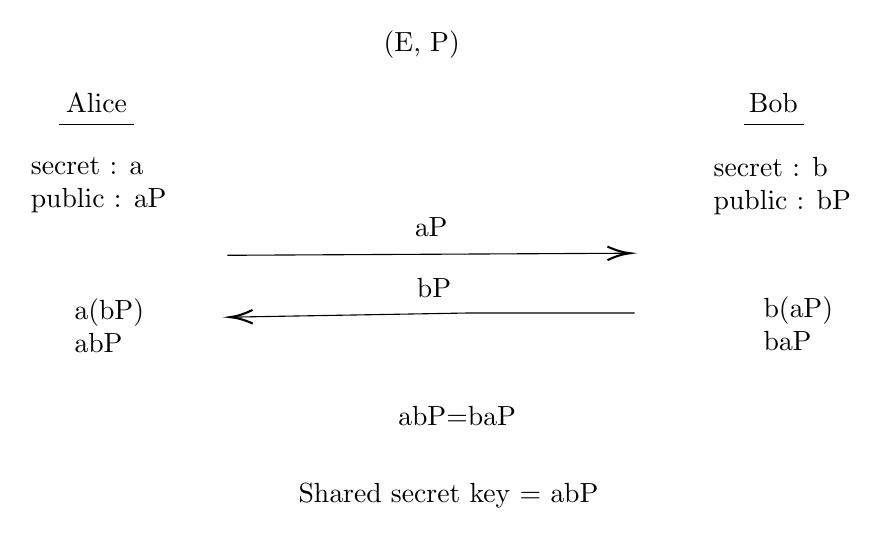
\begin{tikzpicture}[x=0.75pt,y=0.75pt,yscale=-1,xscale=1]
%uncomment if require: \path (0,300); %set diagram left start at 0, and has height of 300

%Straight Lines [id:da1435011466169438] 
\draw    (137,64.4) -- (173,64.4) ;
%Straight Lines [id:da7210376025319416] 
\draw    (467,64.4) -- (496,64.4) ;
%Straight Lines [id:da03246958013588985] 
\draw    (218,127.4) -- (319.21,126.88) -- (410,126.41) ;
\draw [shift={(412,126.4)}, rotate = 179.7] [color={rgb, 255:red, 0; green, 0; blue, 0 }  ][line width=0.75]    (10.93,-3.29) .. controls (6.95,-1.4) and (3.31,-0.3) .. (0,0) .. controls (3.31,0.3) and (6.95,1.4) .. (10.93,3.29)   ;
%Straight Lines [id:da47817176973288045] 
\draw    (414.2,155.2) -- (334.2,155.2) -- (221.2,157.17) ;
\draw [shift={(219.2,157.2)}, rotate = 359] [color={rgb, 255:red, 0; green, 0; blue, 0 }  ][line width=0.75]    (10.93,-3.29) .. controls (6.95,-1.4) and (3.31,-0.3) .. (0,0) .. controls (3.31,0.3) and (6.95,1.4) .. (10.93,3.29)   ;

% Text Node
\draw (139,48) node [anchor=north west][inner sep=0.75pt]   [align=left] {Alice};
% Text Node
\draw (468,48) node [anchor=north west][inner sep=0.75pt]   [align=left] {Bob};
% Text Node
\draw (122,79) node [anchor=north west][inner sep=0.75pt]   [align=left] {secret : a\\public : aP};
% Text Node
\draw (292,18) node [anchor=north west][inner sep=0.75pt]   [align=left] {(E, P)};
% Text Node
\draw (451,79) node [anchor=north west][inner sep=0.75pt]   [align=left] {secret : b\\public : bP};
% Text Node
\draw (307,108) node [anchor=north west][inner sep=0.75pt]   [align=left] {aP};
% Text Node
\draw (308,137) node [anchor=north west][inner sep=0.75pt]   [align=left] {bP};
% Text Node
\draw (143,147) node [anchor=north west][inner sep=0.75pt]   [align=left] {a(bP)\\abP};
% Text Node
\draw (475,146) node [anchor=north west][inner sep=0.75pt]   [align=left] {b(aP)\\baP};
% Text Node
\draw (299,199) node [anchor=north west][inner sep=0.75pt]   [align=left] {abP=baP};
% Text Node
\draw (251,236) node [anchor=north west][inner sep=0.75pt]   [align=left] {Shared secret key = abP};


\end{tikzpicture}
\end{center}
In the above scenario, E and P were public while a, b were secret. Since a,b,P are all discrete, we can find aP(a times P), bP(b times P) and so on. Since they are discrete, abP and baP are same. Since both Alice and Bob finally reached the same point on the curve, they have successfully exchanged messages.\\
\textbf{Note:} Security of ECDH depends on the fact that finding xP from P is computationally difficult. This hard problem is known as \textbf{Discrete log problem on EC}.
\underline{Note:} We plot and see the elliptic curve calculations on Jupyter Notebook. We can get the codes from the website called Sagehelp.
\subsubsection{Elliptic Curve Digital Signature Algorithm(ECDSA)}
Let us first recall that:\\
\textbf{RSA-Signature}:\\
\begin{itemize}
    \item RSA Encryption/Decryption:\\
    Encryption : c = $x^e$ mod n\\
    Decryption : x = $c^d$ mod n\\

    \item Signature :\\
    Signature : s = $x^d$ mod n\\
    Verification : x = $s^e$ mod n\\
\end{itemize}
In ECDSA, we have (E, P) as public keys.\\
\begin{center}
    Secret Key : a\\
    Public Key : aP\\
\end{center}
Here, we need 
\begin{itemize}
    \item elliptic curve EC
    \item a base point-G on the curve. G is such that there exists a large prime number n, such that
\end{itemize}
\begin{center}
    $n\cdotG = 0$\\
    $\implies$ $(n-1)G\ \boxed{+} G\ =\ nG$\\
\end{center}
\begin{center}
    Secret Key : $d_A$\\
    Public Key $Q_A$ : $d_A$
\end{center}
Now let us see a scenarios between Alice and Bob:
\begin{center}
    

\tikzset{every picture/.style={line width=0.75pt}} %set default line width to 0.75pt        

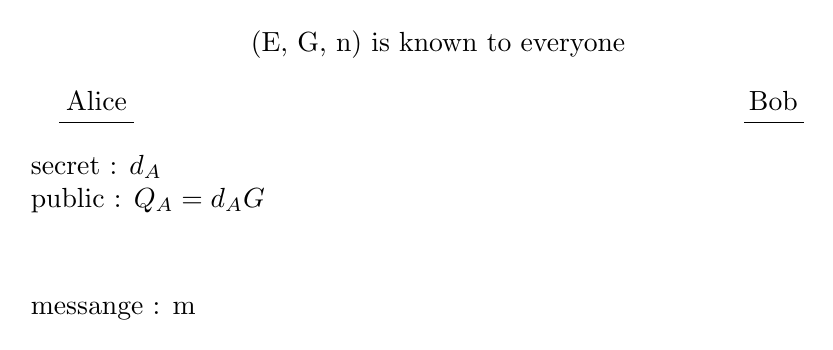
\begin{tikzpicture}[x=0.75pt,y=0.75pt,yscale=-1,xscale=1]
%uncomment if require: \path (0,300); %set diagram left start at 0, and has height of 300

%Straight Lines [id:da1435011466169438] 
\draw    (137,64.4) -- (173,64.4) ;
%Straight Lines [id:da7210376025319416] 
\draw    (467,64.4) -- (496,64.4) ;

% Text Node
\draw (139,48) node [anchor=north west][inner sep=0.75pt]   [align=left] {Alice};
% Text Node
\draw (468,48) node [anchor=north west][inner sep=0.75pt]   [align=left] {Bob};
% Text Node
\draw (122,79) node [anchor=north west][inner sep=0.75pt]   [align=left] {secret : $d_A$\\public : $Q_A = d_AG$};
% Text Node
\draw (228,19) node [anchor=north west][inner sep=0.75pt]   [align=left] {(E, G, n) is known to everyone};
% Text Node
\draw (122,150) node [anchor=north west][inner sep=0.75pt]   [align=left] {messange : m};


\end{tikzpicture}
\end{center}
Let us now see the process of Signature:
\begin{enumerate}
    \item e = Hash(m)
    \item \zbar $\rightarrow\ L_n$ leftmost bits of e when $L_n$ is the bit length of n
    \item K $\rightarrow$ randomly from [1, n-1]
    \item $(x_1, y_1)$ = K$\cdot$G\\
    \item r = $x_1$ mod n\\
    if r = 0 then go to step 3\\
    \item $s\ =\ K^{-1}$ [ \zbar + $r \cdot d_A $  ] mod n\\
    if s = 0, then go to step 3
    \item Signature (r, s) on message m
\end{enumerate}
Let us now see verification of ECDSA performed by Bob:
\begin{enumerate}
    \item $Q_A$ is not equal to 0
    \item $Q_A$ lies on the curve EC or not
    \item $n\times Q_A$ = $n \cdot (d_A \cdot G)$ = $d_A \cdot (n \cdot G)$ = 0
\end{enumerate}
Bob received the message(r, s). To verify, we must follow these steps:
\begin{enumerate}
    \item verify r, s $\in$ [1, n-1]
    \item e = Hash(m)
    \item \zbar $\ \rightarrow\ L_n$ leftmost bits of e
    \item $u_1 \ =\ $ \zbar$\cdot s^{-1}$ mod n\\
    $u_2\ =\ r \cdot s^{-1}$ mod n
    \item $(x_2, y_2)\ =\ u_1G\ +\ u_2Q_A$\\
    if $(x_2, y_2)$ = 0, then signature is invalid. Here addition is addition on the curve.
    \item If r $\equiv\ x_2$ mod n, then signature is valid, otherwise invalid.
\end{enumerate}
Let us see the proof now:\\
\begin{center}
    c = $u_1G\ +\ u_2Q_A$\\
    c = $u_1G\ +\ u_2d_AG$\\
    c = $(u_1\ +\ u_2d_A)$G\\
    c = (\zbar$\cdots^{-1}\ +\ rs^{-1}d_A)$G\\
    c = (\zbar $\ +\ rd_A)s^{-1}$G\\
    Substituting $s^{-1}$\\
    c = (\zbar $\ +\ r\cdot d_A){(K^{-1}(\zbar\ +\ r\cdot d_A))}^{-1}$G\\
    c = (\zbar $\ +\ r\cdot d_A){(\zbar\ +\ r \cdot d_A)}^{-1}$KG\\
    c = K$\cdot$G
\end{center}
Hence, proved.
\end{document}

















\end{document}
